\chapter{Size Distributions}
\label{sizedistribution}

\section{Delta} \hspace{1pt} \\
\label{sec:Delta}
Choosing \texttt{Delta} as a size distribution simply scales the form factor with a constant value $N$

\vspace{5mm}
\underline{Input Parameters for size distribution \texttt{Delta}:}
\begin{description}
\item[\texttt{N}] particle number density $N$
\end{description}

\clearpage

\section{Uniform distribution} \hspace{1pt} \\

\begin{figure}[htb]
\begin{center}
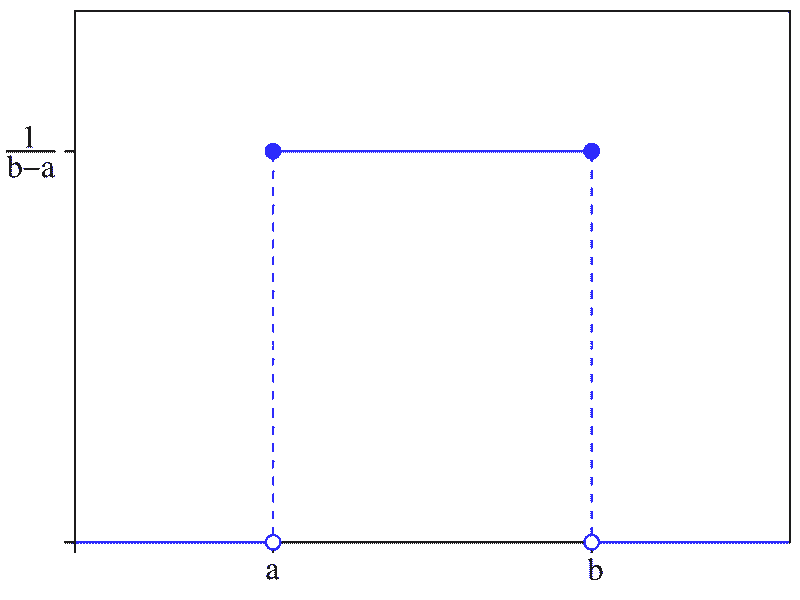
\includegraphics[width=0.744\textwidth,height=0.558\textwidth]{Uniform.png}
\end{center}
\caption{Uniform distribution function. $x_\text{min},x_\text{max} \in
(-\infty,\infty)$, $x_\text{max}>x_\text{min}$, $x_\text{min}\leq x \leq x_\text{max}$} \label{Uniform}
\end{figure}

The uniform distribution defines equal probability over a given range for a continuous distribution.
The support is defined by the two parameters, $x_\text{min}$ and $x_\text{max}$, which are its
minimum and maximum values.

\begin{subequations}
\begin{align}
\text{Uniform}(x\vert N, x_\text{min},x_\text{max}) & =
   \begin{cases}
      \displaystyle \frac{N}{x_\text{max}-x_\text{min}} & \text{for} \quad x_\text{min}\leq x\leq x_\text{max}, \\
      & \\
      \displaystyle 0               & \text{for} \quad x< x_\text{min} \text{~or~} x>x_\text{max}
   \end{cases}
\end{align}
\end{subequations}

\vspace{5mm}
\underline{Input Parameters for size distribution \texttt{Uniform}:}
\begin{description}
\item[\texttt{N}] particle number density $N$
\item[\texttt{Xmin}] minimum value of the distribution ($x_\text{min}$)
\item[\texttt{Xmax}] maximum value of the distribution ($x_\text{max}$)
\end{description}

%%%%%%%%%%%%%%%%%%%%%%%%%%%%%%%%%%%%%%%%%%%%%%%%%%%%%%%%%%%%%%%%%%%%%%%%%%%

\clearpage
\section{Triangular distribution} ~\\

\begin{figure}[htb]
\begin{center}
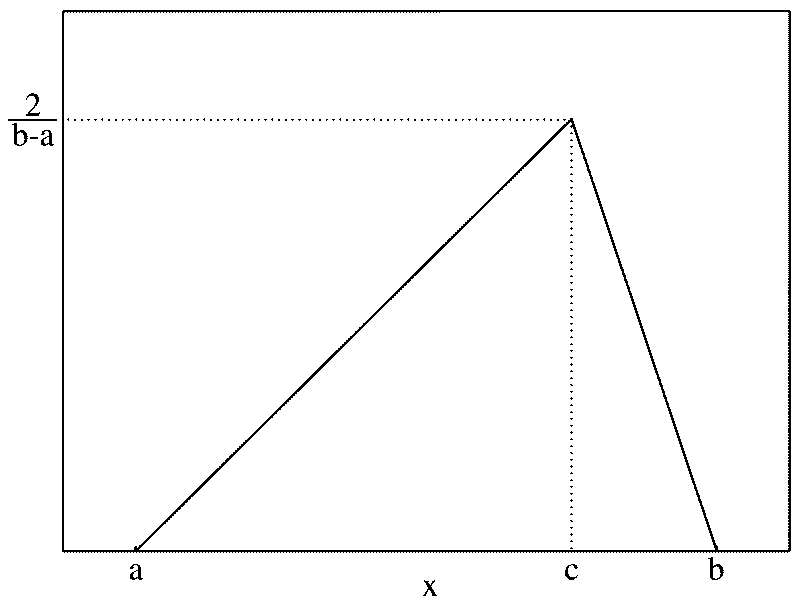
\includegraphics[width=0.744\textwidth,height=0.558\textwidth]{Triangular.png}
\end{center}
\caption{Triangular distribution function.
$x_\text{min},x_\text{mode},x_\text{max} \in (-\infty,\infty)$,
$x_\text{max}>x_\text{min}$,
$x_\text{min}\leq x_\text{mode}\leq x_\text{max}$,
$x_\text{min}\leq x \leq x_\text{max}$}
\label{Triangular}
\end{figure}

\begin{subequations}
\begin{multline}
\text{Triangular}(x\vert x_\text{min},x_\text{max},x_\text{mode})   =  \\
   \begin{cases}
      \displaystyle \frac{2(x-x_\text{min})}{(x_\text{max}-x_\text{min})(x_\text{mode}-x_\text{min})} & \text{for} \quad x_\text{min}<x\leq x_\text{mode} \\
      & \\
      \displaystyle \frac{2(x_\text{max}-x)}{(x_\text{max}-x_\text{min})(x_\text{max}-x_\text{mode})} & \text{for} \quad x_\text{mode}<x\leq x_\text{max}
   \end{cases}
\end{multline}
\end{subequations}

%%%%%%%%%%%%%%%%%%%%%%%%%%%%%%%%%%%%%%%%%%%%%%%%%%%%%%%%%%%%%%%%%%%%%%%%%%%%%%%%

\clearpage
\section{Log-Normal distribution}
\label{sect:LogNormSD}
\begin{figure}[htb]
\begin{center}
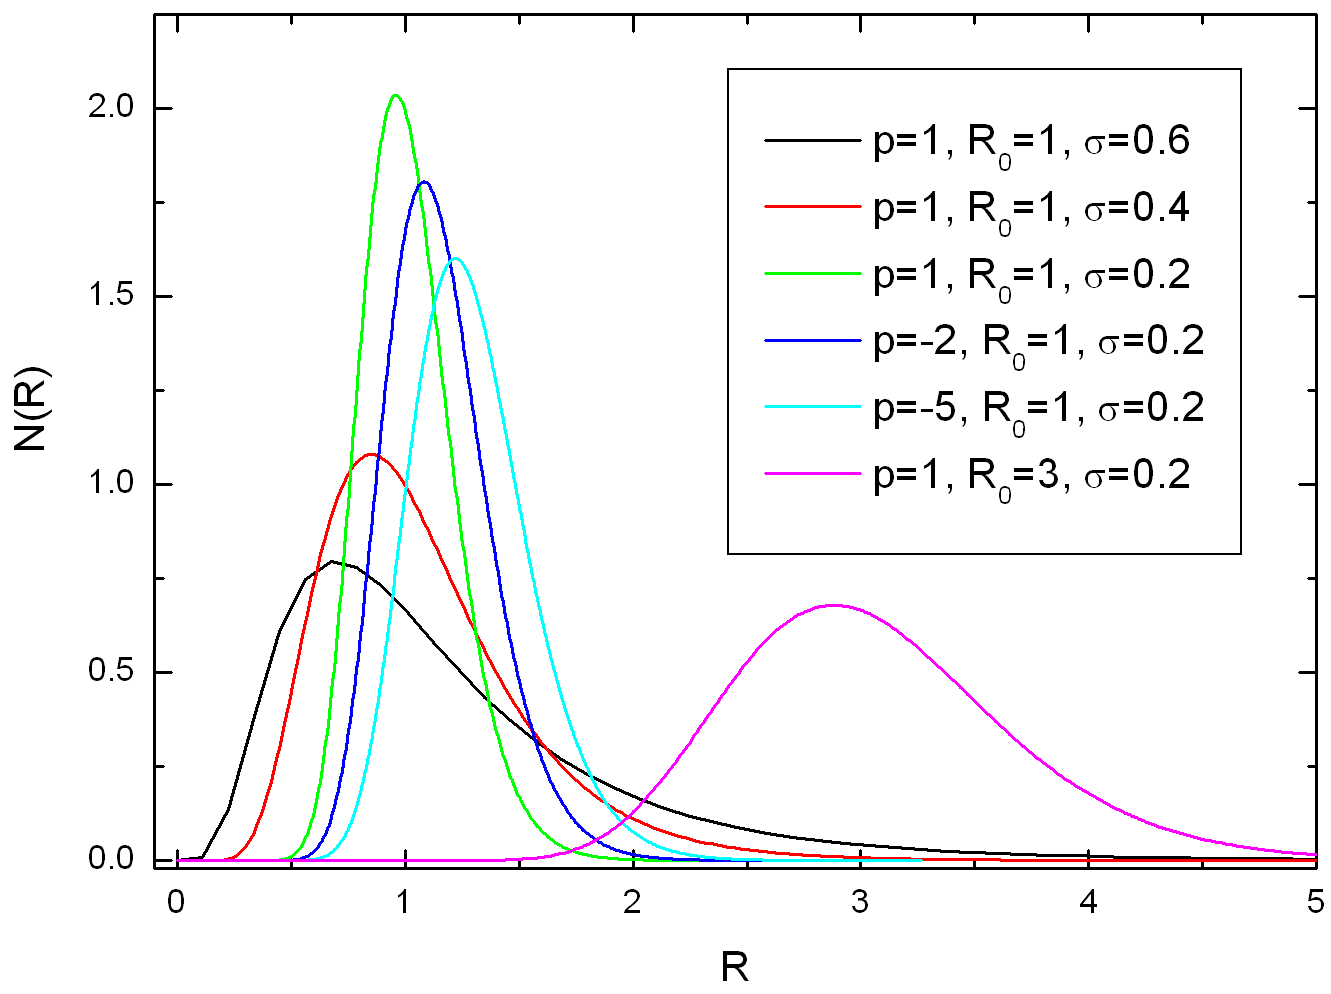
\includegraphics[width=0.878\textwidth,height=0.656\textwidth]{LogNorm.png}
\end{center}
\caption{LogNormal distribution function ($R_0=1$ and $p=1$ has
been been set both to one here). Valid parameter ranges: $R \in
(0,\infty)$, $R_0 \in (0,\infty)$, $\sigma\geq 0$, $p \in
(-\infty,\infty)$} \label{NogNormal}
\end{figure}

The \texttt{LogNorm} distribution is a continuous distribution in
which the logarithm of a variable has a normal distribution.
\begin{subequations}
\begin{align}
\text{LogNorm}(X,\mu,\sigma,p) &=  \frac{N}{c_\text{LN}}
                                    \frac{1}{X^{p}}\,
                                    \exp\!\!\left(-\frac{\ln(X/\mu)^2}{2\sigma^2}\right) \\
c_\text{LN} &= \sqrt{2\pi}\,\sigma \,\mu^{1-p}
\,\exp\!\!\left((1-p)^2\frac{\sigma^2}{2}\right)
\label{eq:LogNormal}
\end{align}
\end{subequations}
where $\sigma$ is the width parameter, $p$ a shape parameter, $\mu$ is the location parameter.
$c_\text{LN}$ is choosen so that $\int_0^\infty\! \text{LogNorm}(X,\mu,\sigma,p)\,dX = N$
The mode of the distribution $X_\text{mode}$ and the variance
$\text{Var}(X)$ are defined as
\begin{align}
X_\text{mode} &= \mu e^{-p \sigma^2} \\
\text{Var}(X) &= \mu ^2 \left(e^{\sigma^2}-1\right) e^{(3-2 p) \sigma^2}
\end{align}
and the $m^\text{th}$ moment $\langle X^m\rangle$ of the \texttt{LogNorm} distribution as
\begin{align}
\langle X^m\rangle = \frac{\int X^m\, \textrm{LogNorm}(X)\, dX}{\int \textrm{LogNorm}(X)\, dX} =
\mu^m \, e^{\frac{1}{2} \sigma^2 m (2 - 2 p + m)}.
\label{eq:nMoment:LogNormal}
\end{align}
%%%%%%%%%%%%%%%%%%%%%%%%%%%%%%%%%%%%%%%%%%%%%%%%%%%%%%%%%%%%%%%%%%%%%%%%%%%%%%

\clearpage
\section{Schulz-Zimm (Flory) distribution}

\begin{figure}[htb]
\begin{center}
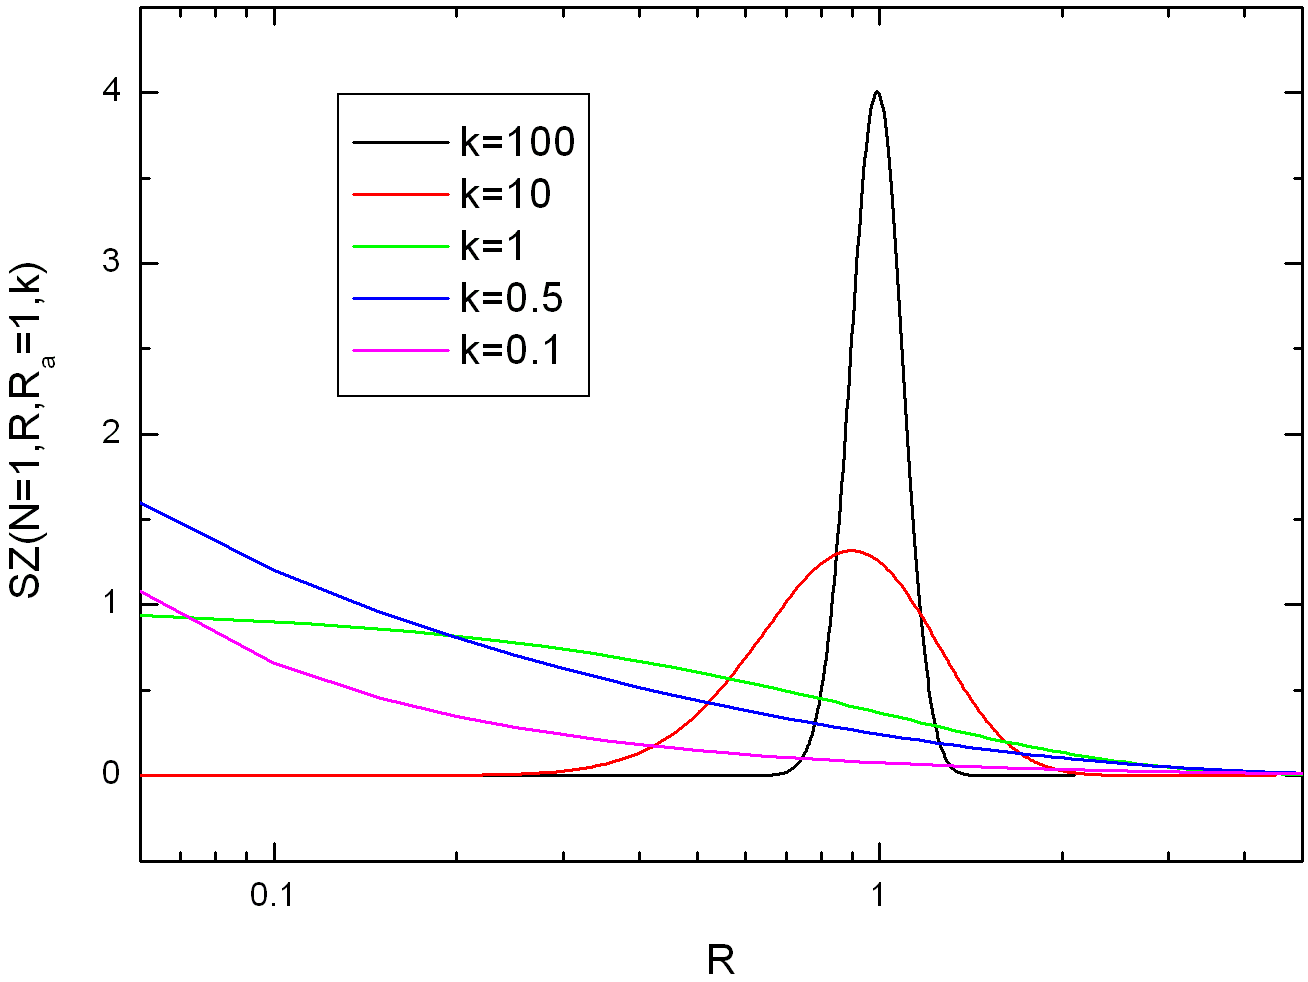
\includegraphics[width=0.876\textwidth,height=0.658\textwidth]{SZ.png}
\end{center}
\caption{The $\text{SZ}(X,N,X_a,k)$ distribution function. Valid
parameter ranges: $X \in [0,\infty)$, $X_a \in (0,\infty)$,
$k=X_a^2/\sigma^2 > 0$} \label{NogNormal}
\end{figure}

A function commonly used to present polymer molecular weight distributions is the Schulz-Zimm function
\begin{equation}
\textrm{SZ}_n(X,N,X_a,k) =  \frac{N}{X_a}
\left(\frac{X}{X_a}\right)^{k-1}
\frac{k^k\exp(-kX/X_a)}{\Gamma(k)}
\label{eq:SZn(M)}
\end{equation}
~\\
$\text{SZ}_n(X,N,X_a,k)$ is normalized so that $\int_0^\infty\!
\text{SZ}_n(X,N,X_a,k)\,dX = N$.
In polymer science $X$ would be the molecular weight $M$,
$\overline{M}_n=X_a$, and $\overline{M}_w=\overline{M}_n\frac{k+1}{k}$,
and $\Gamma(k)$ is the gamma function.
The above form (\ref{eq:SZn(M)}) gives the number distribution.
Its mode, mean, variance and $m^\textrm{th}$-moment are given by
\begin{subequations}
\begin{align}
X_\textrm{mode} &= X_a \left(1-\frac{1}{k}\right)\\
X_\textrm{mean} &= X_a \\
\textrm{Var}\left(X\right)=\sigma^2 &= \frac{X_a^2}{k} \\
\left\langle X^m \right\rangle &=
\left(\frac{X_a}{k}\right)^m  \frac{\Gamma \left(k+m\right)}{\Gamma (k)}
\label{eq:SZstatparam}
\end{align}
\end{subequations}
The corresponding weight distribution is
\begin{equation}
\textrm{SZ}_w(X,N,X_a,k) = \frac{X}{X_a}\textrm{SZ}_n(X,N,X_a,k)
=  \frac{N X^k \left(\frac{k}{X_a}\right)^{k+1} e^{-\frac{kX}{X_a}}}{\Gamma(k+1)}
\end{equation}
~\\
Also $\textrm{SZ}_w(X,N,X_a,k)$ is normalized so that $\int_0^\infty\!
\textrm{SZ}_w(X,N,X_a,k)\,dX = N$.
The mode, mean, variance and
$m^\textrm{th}$-moment of the weight distribution are given by
\begin{subequations}
\begin{align}
X_\textrm{mode} &= X_a\\
X_\textrm{mean} &= X_a \frac{1+k}{k}\\
\textrm{Var}\left(X\right)&=\sigma^2 = X_a^2\frac{1+k}{k^2} \\
\left\langle X^m \right\rangle &=
\left(\frac{X_a}{k}\right)^m  \frac{\Gamma \left(k+m+1\right)}{\Gamma \left(k+1\right)}
\label{eq:SZFstatparam}
\end{align}
\end{subequations}

%%%%%%%%%%%%%%%%%%%%%%%%%%%%%%%%%%%%%%%%%%%%%%%%%%%%%%%%%%%%%%%%%%%%%%%%%%%%%%%%%


\clearpage
\section{Gamma distribution}

The Gamma distribution is a two parameter continuous distribution with
a scale parameter $\theta$ and a shape parameter $k$.
\begin{equation}
\text{gammaSD}(x,N,x_\text{mode},\sigma) =  \frac{N}{\theta}
\left(\frac{x}{\theta}\right)^{k-1}
\frac{\exp(-x/\theta)}{\Gamma(k)} \label{GammaSDEq}
\end{equation}
The mean $x_\text{mean}$, mode $x_\text{mode}$ and variane $\sigma^2$
of the distribution are given by
\begin{align}
x_\text{mean}   &= k\theta \\
x_\text{mode}   &= (k-1)\theta \text{ for } k\geq 1 \\
\sigma^2        &= k\theta^2
\end{align}
The gamma distribution is more flexible than the exponential or $\xi^2$ distribution
function which are special cases of the gamma distribution function.
When $k$ is large, the gamma distribution closely approximates a normal distribution
with the advantage that the gamma distribution has density only for positive real
numbers. For small values of $k$ the distribution becomes a right tailed distribution.

The $m^\text{th}$ moment $\langle X^m\rangle$ of the size distribution is given by
\begin{align}
\langle X^m\rangle = \theta^m \frac{\Gamma(k+m)}{\Gamma(k)} .
\end{align}
In the present version the Gamma distribution is parametrised as a function
of the mode and variance, i.e.
with
\begin{align}
k=\frac{x_\text{mode} \sqrt{x_\text{mode}^2+4
   \sigma^2}+x_\text{mode}^2+2 \sigma ^2}{2 \sigma^2}
\end{align}
 and
\begin{align}
 \theta = \frac{1}{2}
   \left(\sqrt{x_\text{mode}^2+4 \sigma ^2}-x_\text{mode}\right)
\end{align}
$\text{gammaSD}(R,N,R_m,\sigma)$ is normalized so that
$\int_0^\infty\! \text{gammaSD}(R,N,R_m,\sigma)\,dR = N$.

\vspace{5mm}
\noindent \underline{Input Parameters for model \texttt{Sphere}:}
\begin{description}
\item[\texttt{N}]  $N$
\item[\texttt{mode}] mod of the distribution (maximum, most probable size) $x_\text{mode}>0$
\item[\texttt{sigma}] width parameter $\sigma>0$. The variance of the distribution is $\sigma^2$.
\end{description}

\noindent\underline{Note:}
\begin{itemize}
\item The parameters \texttt{mode} and \texttt{sigma} needs to be positive.
\end{itemize}

\begin{figure}[htb]
\begin{center}
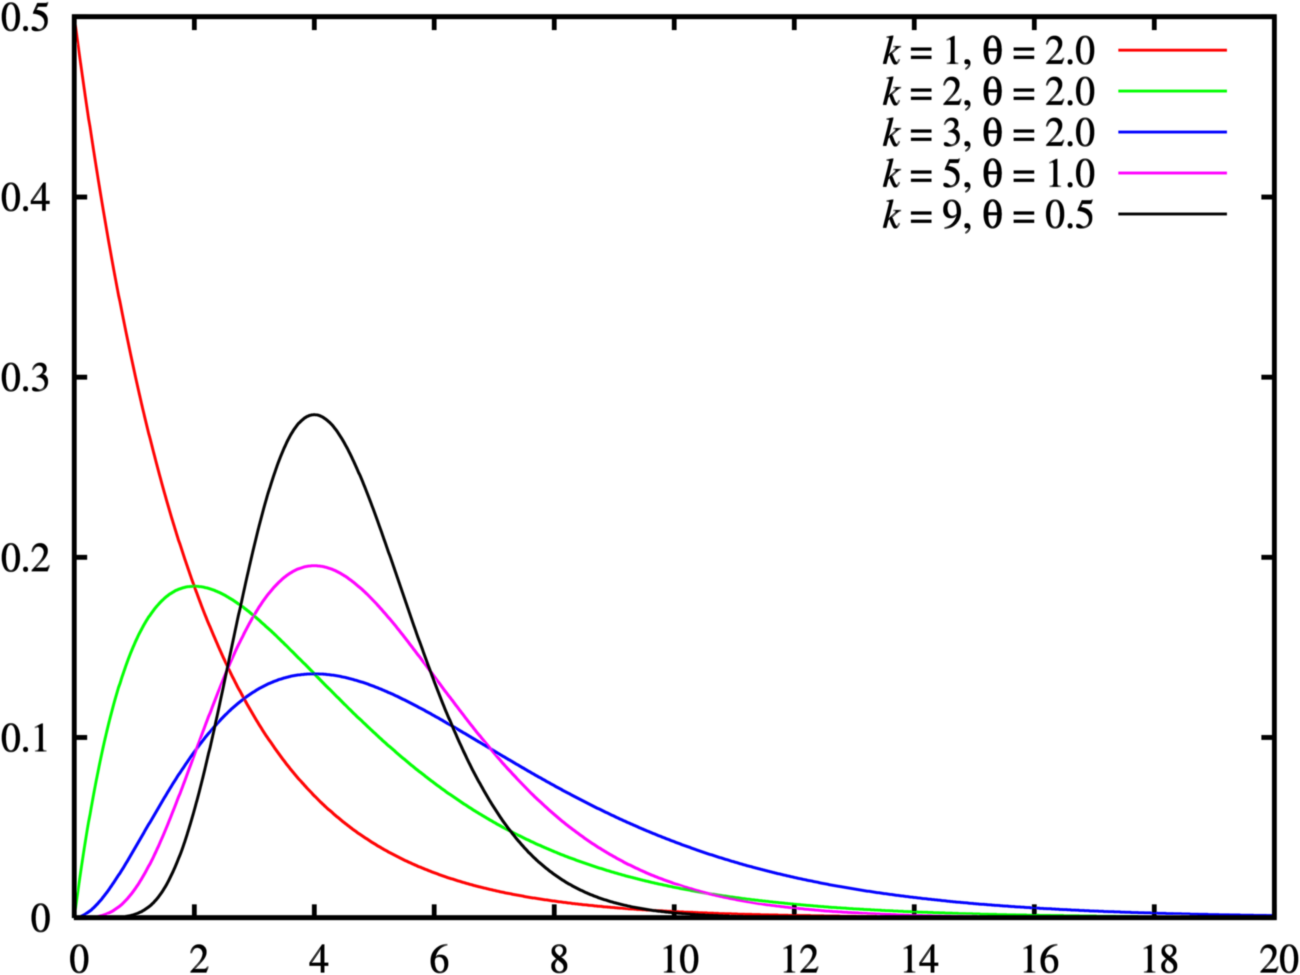
\includegraphics[width=0.8\textwidth,height=0.6\textwidth]{Gamma_distribution_pdf.png}
\end{center}
\caption{The $\text{gammaSD}(R,N,x_{mode},\sigma)$ distribution
function.
Valid parameter ranges:
$x\in [0,\infty)$,
$x_\text{mode} \in (0,\infty)$,
$\sigma > 0$}
\label{GammaSD}
\end{figure}
%%%%%%%%%%%%%%%%%%%%%%%%%%%%%%%%%%%%%%%%%%%%%%%%%%%%%%%%%%%%%%%%%%%%%%%%%%%%%%%%%%%%%%%%%%%%%

\clearpage
\section{PearsonIII distribution}

The Pearson distribution is a family of probability distributions
that are a generalisation of the normal distribution. The Pearson
Type III distribution is given by the probability density function
\BE
    f(x) = \frac{1}{\beta\,\Gamma(p)} \left(\frac{x-\alpha}{\beta}\right)^{p-1} e^{-(x-\alpha)/\beta}, \!
\EE where $x \in [\alpha,\infty)$ and $\alpha$, $\beta$ and $p$
are parameters of the distribution with $\beta > 0$ and $p > 0$
(Abramowitz and Stegun 1954, p. 930). Here, $\Gamma ()$ denotes
the Gamma function.
\begin{itemize}
%\item Characteristic function:
%$$
%    e^{\imath\alpha t}(1 - \imath\beta t)^{-p}
%$$
\item Mean:
$$
    \alpha + p\beta
$$
\item Variance:
$$
    p\beta^2
$$
\item Skewness:
$$
    \frac{2}{\sqrt{p}}
$$
\item Kurtosis:
$$
    \frac{6}{p}
$$
\end{itemize}
The Pearson Type III distribution is identical to the Gamma
distribution (\ref{GammaSDEq}). When $\alpha=0$, $\beta=2$, and
$p$ is half-integer, the Pearson Type III distribution becomes the
$\chi^2$ distribution of $2p$ degrees of freedom.

%%%%%%%%%%%%%%%%%%%%%%%%%%%%%%%%%%%%%%%%%%%%%%%%%%%%%%%%%%%%%%%%%%%%%%%%%%%%%%%%%%%%%

\clearpage
\section{Gauss distribution}

\begin{figure}[htb]
\begin{center}
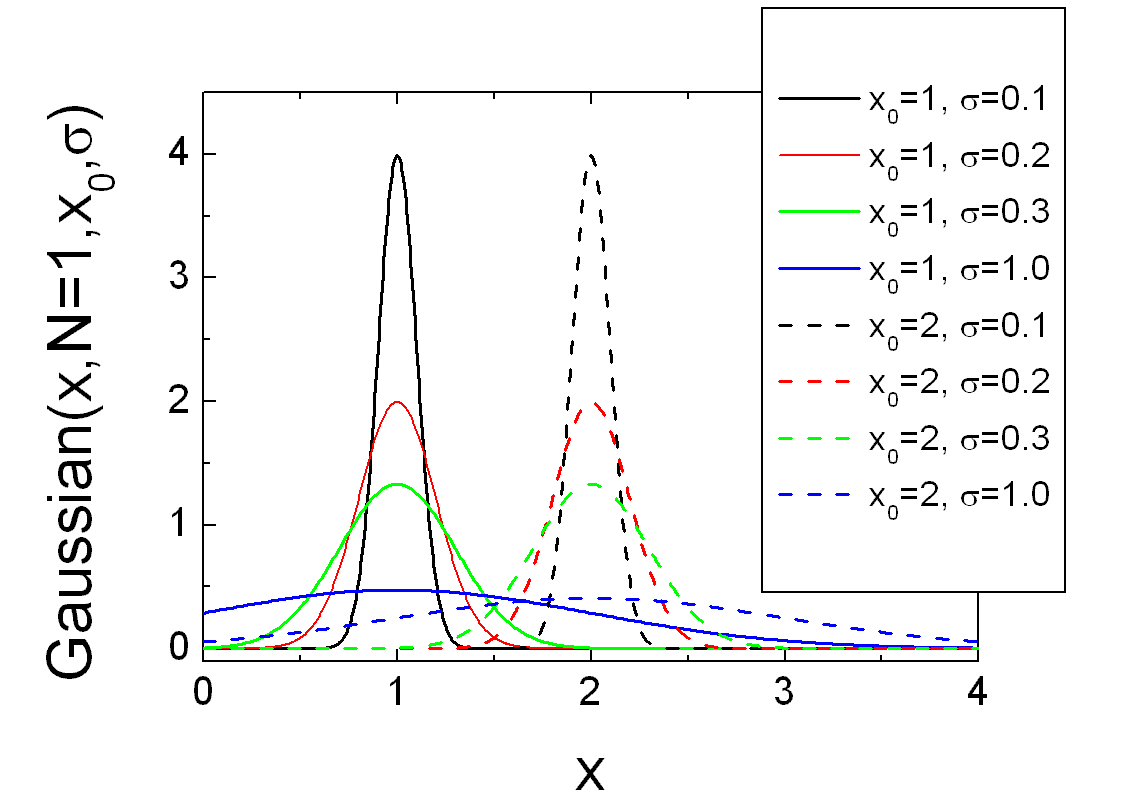
\includegraphics[width=0.873\textwidth,height=0.653\textwidth]{GaussSD.png}
\end{center}
\caption{Normal or Gauss distribution function ($R_0=\mu=0$ has
been chosen in the plot). Valid parameter ranges: $R \in
(0,\infty)$, $R_0 \in (-\infty,\infty)$, $\sigma>0$}
\label{NormalDistr}
\end{figure}

\begin{subequations}
\begin{align}
\text{Gauss}(R,N,\sigma,R_0)&= \frac{N}{c_\text{Gauss}}
e^{-\frac{\left(R-R_0\right)^2}{2\sigma^2}}
\label{eq:GaussDistribution} \\
c_\text{Gauss} &=\sqrt{\frac{\pi}{2}}\sigma\left(1 +
\text{erf}\left(\frac{R_0}{\sqrt{2}\sigma}\right) \right)
\end{align}
\end{subequations}
$c_\text{Gauss}$ is choosen so that $\int_0^\infty\!
\text{Gauss}(R,\sigma,R_0)\,dR = N$

%%%%%%%%%%%%%%%%%%%%%%%%%%%%%%%%%%%%%%%%%%%%%%%%%%%%%%%%%%%%%%%%%%%%%%%%%%%%%%%%%%%%%%%%%

\clearpage
\section{Generalized exponential distribution (GEX)}

\begin{subequations}
\begin{align}
\text{GEX}(R,\beta,\lambda,\gamma))&= N
\frac{\beta}{\gamma}\left(\frac{x}{\gamma}\right)^{\lambda+1}
\frac{e^{-(x/\gamma)^{\beta}}}{\Gamma  \left( {\frac
{\lambda+2}{\beta}} \right)}
\end{align}
\end{subequations}

%%%%%%%%%%%%%%%%%%%%%%%%%%%%%%%%%%%%%%%%%%%%%%%%%%%%%%%%%%%%%%%%%%%%%%%%%%%%%%%%%%%%%%%%%%%%%%%

\clearpage
\section{Generalized extreme value distribution (GEV)}

\begin{figure}[htb]
\begin{center}
%\includegraphics[width=0.744\textwidth,height=0.558\textwidth]{GEV.bmp}
\end{center}
\caption{The shape parameter  governs the tail behaviour of the
distribution, the sub-families defined by $\xi\to 0$, $\xi > 0$ and
$\xi < 0$ correspond, respectively, to the Gumbel, Fr\'{e}chet and
Weibull families, whose cumulative distribution functions are
reminded below. Gumbel or type I extreme value distribution}
\label{fig:GEVDistr}
\end{figure}
\BE
\text{GEV}(R,\mu,\sigma,\xi) = \frac{N}{c_1} \frac{{e^{- \left( 1+{\frac
{\xi\, \left( R-\mu \right) }{\sigma} } \right) ^{-1/{\xi}}}}}{
\sigma \left( 1+{\frac {\xi\, \left( R-\mu \right) }{\sigma}}
\right) ^{1+ 1/{\xi}} }
\EE
with
\BE
c_1 =
\begin{cases}
1 & \text{for $\xi>0$}\\
1-\exp\left(-\left(1-\frac{\xi\mu}{\sigma}\right)^{-\frac{1}{\xi}}\right) & \text{for $\xi<0$}
\end{cases}
\EE
The shape parameter $\xi$ governs the tail behaviour of the
distribution, the sub-families defined by $\xi\to 0$, $\xi > 0$ and
$\xi < 0$ correspond, respectively, to the Gumbel, Fr\'{e}chet and
Weibull families, whose cumulative distribution functions are
reminded below.
\begin{itemize}
\item Gumbel or type I extreme value distribution
$$
   F(x;\mu,\sigma)=e^{-e^{-(x-\mu)/\sigma}}\;\;\; for\;\; x\in\mathbb R
$$
\item Fr\'{e}chet or type II extreme value distribution
$$
    F(x;\mu,\sigma,\alpha)=\begin{cases} 0 & x\leq \mu \\ e^{-((x-\mu)/\sigma)^{-\alpha}} & x>\mu \end{cases}
$$

\item Weibull or type III extreme value distribution
$$
    F(x;\mu,\sigma,\alpha)=\begin{cases} e^{-(-(x-\mu)/\sigma)^{-\alpha}} & x<\mu \\ 1 & x\geq \mu \end{cases}
$$
where $\xi > 0$ and $\xi > 0$

Remark I: For reliability issues the Weibull dist ribution is used
with the variable $t = \mu - x$, the time, which is strictly
positive. Thus the support is positive - in contrast to the use in
extreme value theory.

Remark II: Be aware of an important distinctive feature of the
three extreme value distributions: The support is either
unlimited, or it has an upper or lower limit.
\end{itemize}
\begin{itemize}
\item Parameters\\
  $\mu \in [-\infty,\infty]$ \, location (real)\\
  $\sigma \in (0,\infty]$ \, scale (real)\\
  $\xi\in [-\infty,\infty]$\, shape (real)
\item Support\\
  $x>\mu-\sigma/\xi\,\;(\xi > 0)$ \\
  $x<\mu-\sigma/\xi\,\;(\xi < 0)$ \\
  $x \in [-\infty,\infty]\,\;(\xi = 0)$
\end{itemize}
[1]
\verb"http://en.wikipedia.org/wiki/Generalized_extreme_value_distribution"

%%%%%%%%%%%%%%%%%%%%%%%%%%%%%%%%%%%%%%%%%%%%%%%%%%%%%%%%%%%%%%%%%%%%%%%%%%%%%%

\clearpage
\section{Maxwell distribution}

\begin{figure}[htb]
\begin{center}
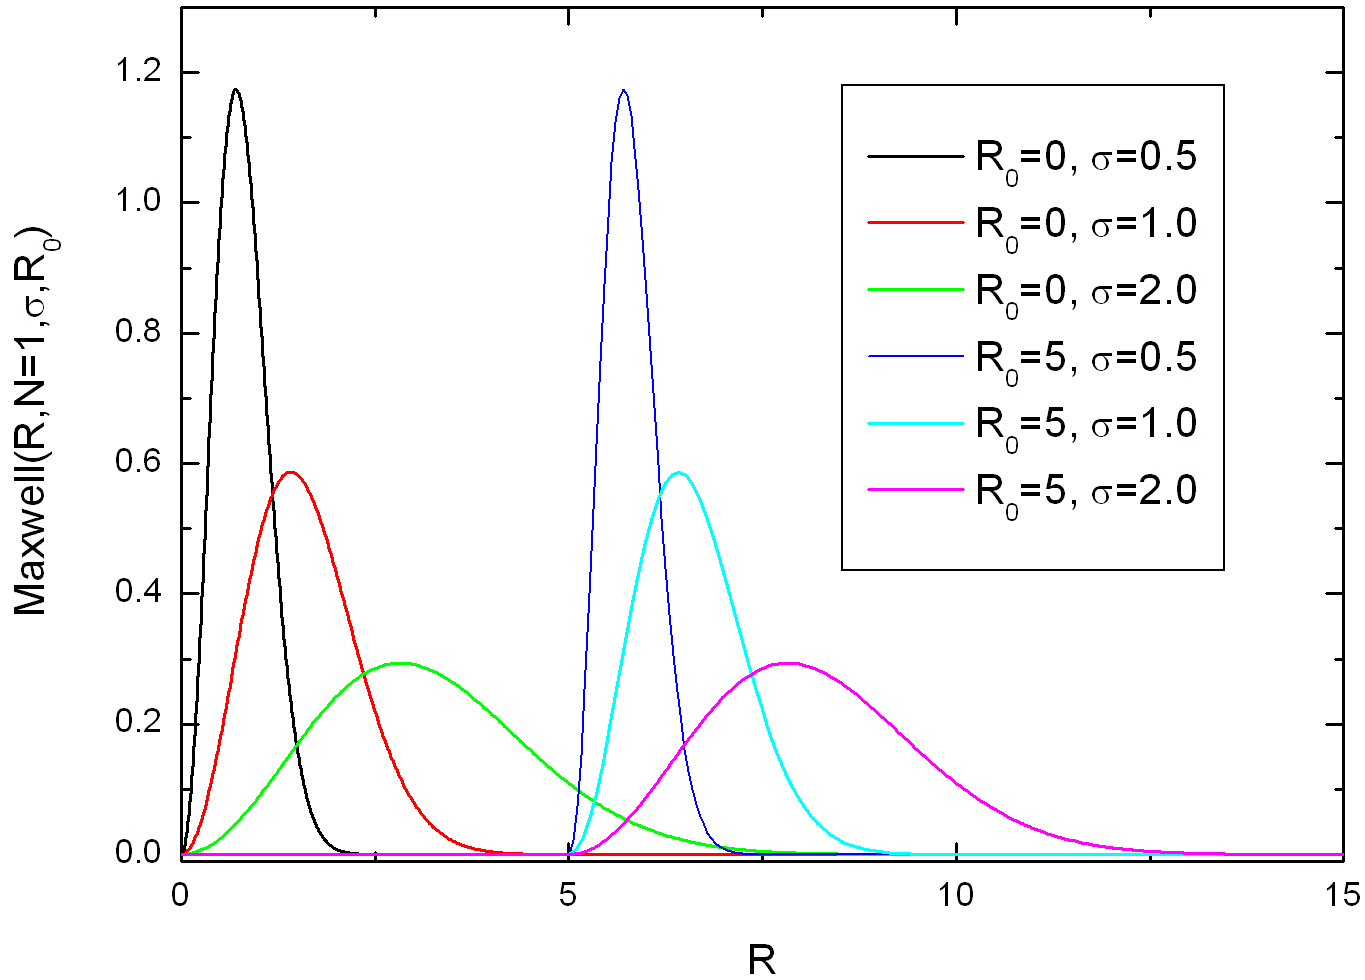
\includegraphics[width=0.874\textwidth,height=0.627\textwidth]{Maxwell.png}
\end{center}
\caption{Maxwell distribution function. Valid parameter ranges: $R
\in [0,\infty)$, $R_0\in (-\infty,\infty)$, $\sigma > 0$}
\label{fig:Maxwell}
\end{figure}
\begin{subequations}
\begin{align}
\text{Maxwell}(R,R_0,\sigma) &=
\begin{cases}
\text{if $R \geq R_0$:} &
N \frac{c}{c_\text{mw}} \left(R-R_0\right)^2 e^{-\left(R-R_0\right)^2/(2\sigma^2)}\\
& \\
\text{else:} & 0
\end{cases} \\
& \nonumber \\
c &= \frac{4}{\sqrt{\pi}} \left(2\sigma^2\right)^{-3/2}  \\
& \nonumber \\
c_\text{mw} &=
\begin{cases}
\text{if $R_0 < 0$:} & 1-\frac{1}{\sigma} \sqrt{\frac{2}{\pi}}
\frac{R_0}{\sqrt{\exp\left(R_0^2/\sigma^2\right)}} +
                  \text{erf}\left(\frac{R_0}{\sqrt{2}\sigma}\right)  \\
                  & \\
\text{else:} & 1
\end{cases}
\end{align}
\end{subequations}

%%%%%%%%%%%%%%%%%%%%%%%%%%%%%%%%%%%%%%%%%%%%%%%%%%%%%%%%%%%%%%%%%%%%%%%%%%%%%%%%%%%%%%%%%%%%%

\clearpage
\section{Weibull distribution}

\begin{figure}[htb]
\begin{center}
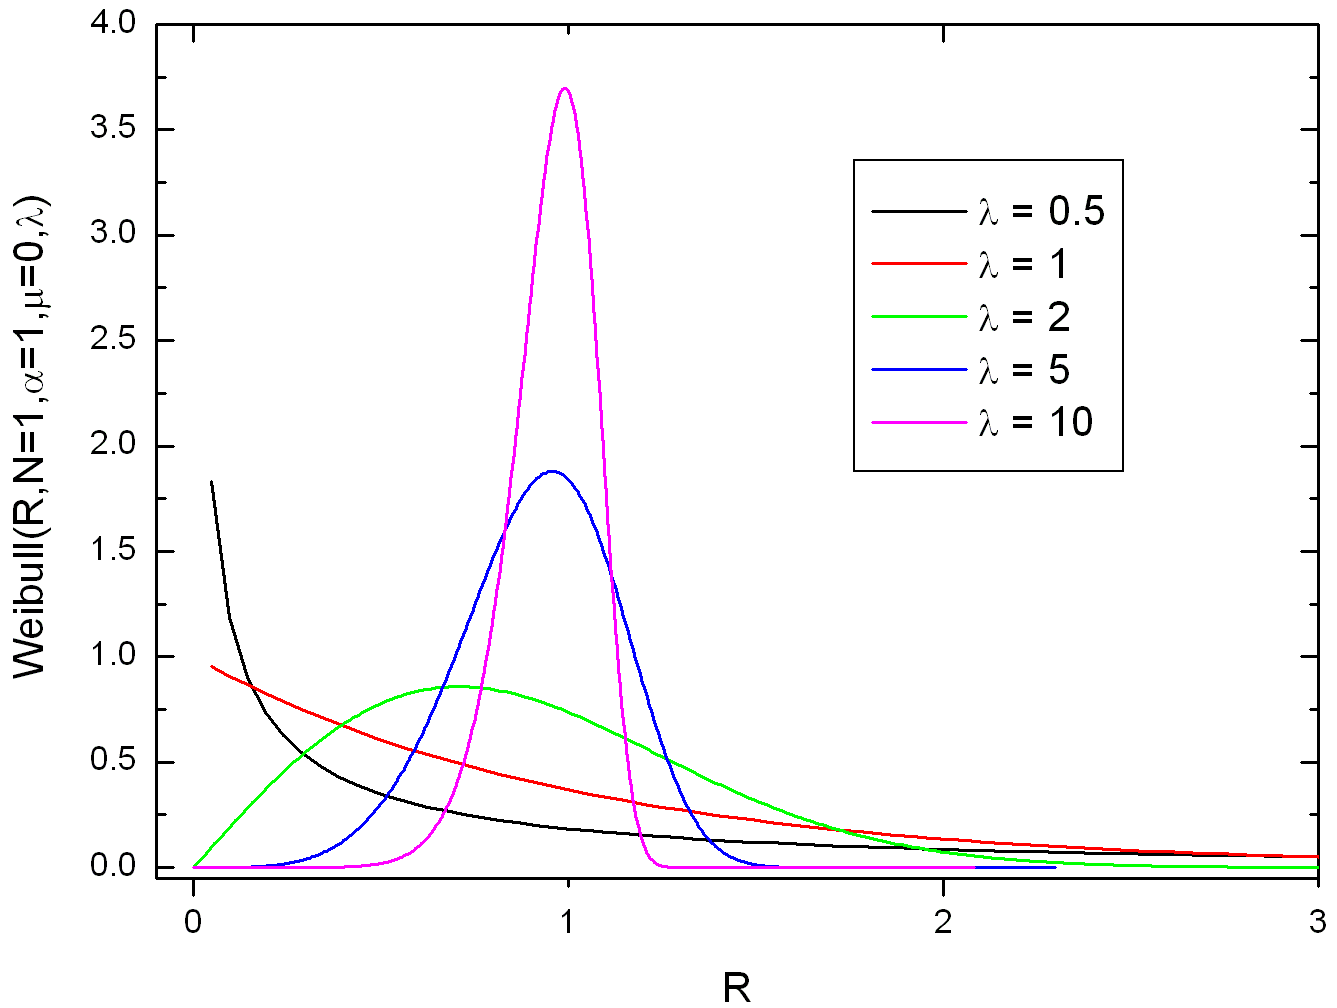
\includegraphics[width=0.869\textwidth,height=0.655\textwidth]{Weibull.png}
\end{center}
\caption{Weibull distribution function ($\mu=0$, $\alpha=1$ has been
chosen in the plot). Valid parameter ranges: $R \in [0,\infty)$,
$\mu \in [0,\infty)$, $\alpha > 0$, $\lambda > 0$}
\label{fig:Weibull}
\end{figure}
\begin{align}
\text{Weibull}(R,\alpha,\lambda,\mu) =
          \frac{N \lambda}{\alpha}
          \left(\frac{R-\mu}{\alpha}\right)^{\lambda-1}
          e^{-\left( \frac{R-\mu}{\alpha} \right)^\lambda}
          e^{-\left(\frac{\mu}{\alpha}\right)^\lambda}
\end{align}
where $\lambda$ is the shape parameter, $\mu$ is the location
parameter and $\alpha$ is the scale parameter.

%%%%%%%%%%%%%%%%%%%%%%%%%%%%%%%%%%%%%%%%%%%%%%%%%%%%%%%%%%%%%%%%%%%%%%%%%%%%%%%%%%%%%%%

\clearpage
\section{fractal size distribution}

\begin{figure}[htb]
\begin{center}
%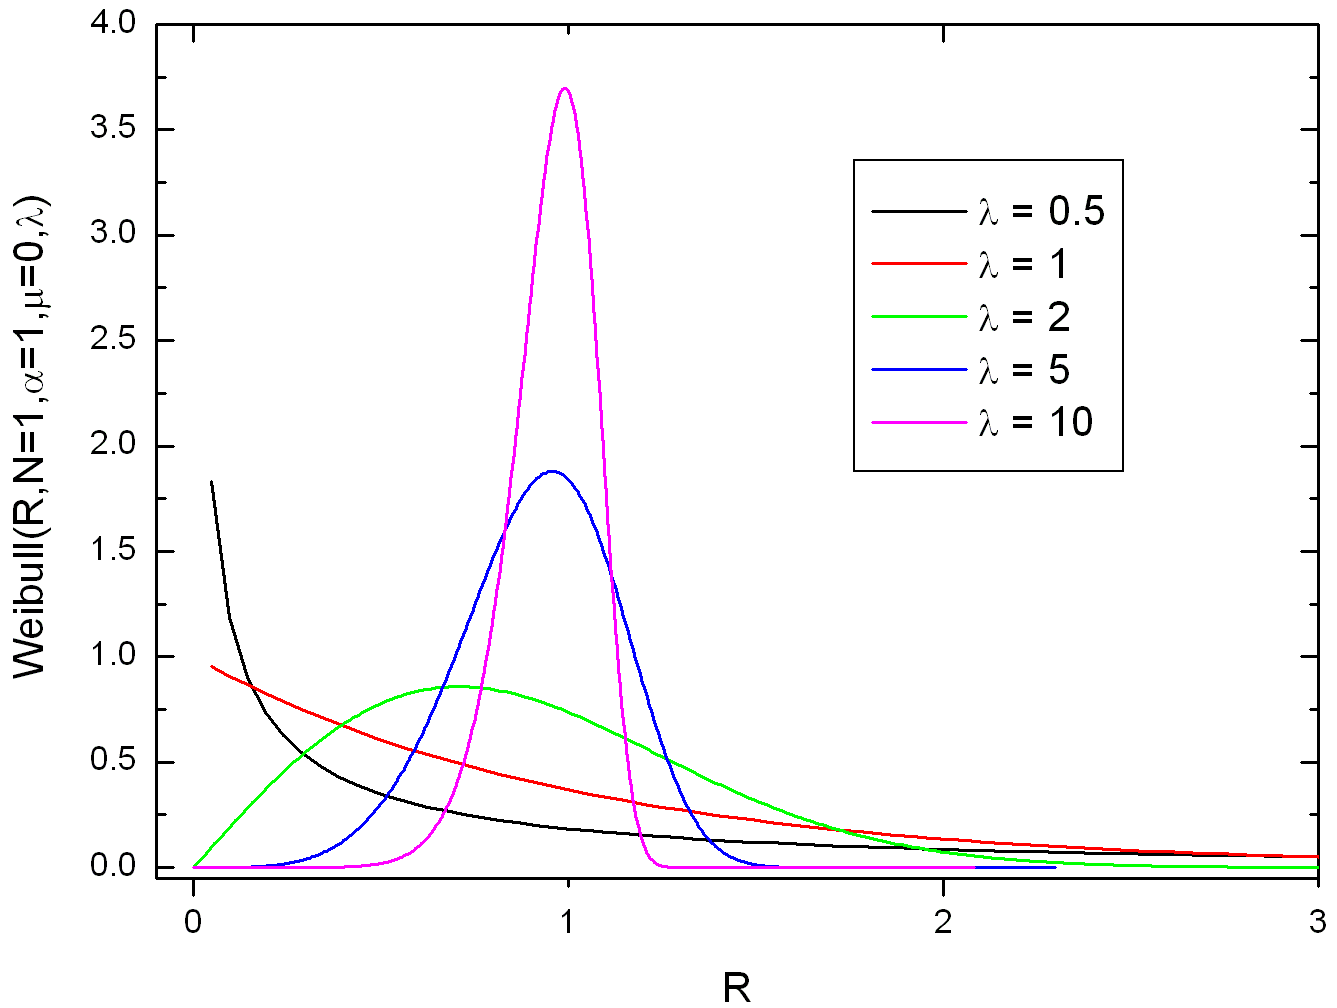
\includegraphics[width=0.869\textwidth,height=0.655\textwidth]{Weibull.bmp}
\end{center}
\caption{fractal size distribution function. Valid parameter ranges:
$R \in [R_\text{min},R_\text{max}]$, $f_D \in (-1,\infty )$,
$R_\text{max} > R_\text{min} > 0$} \label{fig:fractal}
\end{figure}
\begin{equation}
\text{fractalSD}(R,N,R_\text{min},R_\text{max},f_D) = \frac{N f_D
}{R_\text{min}^{-f_D}-R_\text{max}^{-f_D}} \;\; R^{-(1+f_D)}
\end{equation}
